\documentclass{beamer}

%packages:
% \usepackage{tfrupee}
% \usepackage{amsmath}
% \usepackage{amssymb}
% \usepackage{gensymb}
% \usepackage{txfonts}

% \def\inputGnumericTable{}

% \usepackage[latin1]{inputenc}                                 
% \usepackage{color}                                            
% \usepackage{array}                                            
% \usepackage{longtable}                                        
% \usepackage{calc}                                             
% \usepackage{multirow}                                         
% \usepackage{hhline}                                           
% \usepackage{ifthen}
% \usepackage{caption} 
% \captionsetup[table]{skip=3pt}  
% \providecommand{\pr}[1]{\ensuremath{\Pr\left(#1\right)}}
% \providecommand{\cbrak}[1]{\ensuremath{\left\{#1\right\}}}
% %\renewcommand{\thefigure}{\arabic{table}}
% \renewcommand{\thetable}{\arabic{table}}      

\setbeamertemplate{caption}[numbered]{}

\usepackage{enumitem}
\usepackage{tfrupee}
\usepackage{amsmath}
\usepackage{amssymb}
\usepackage{graphicx}
\usepackage{txfonts}

\def\inputGnumericTable{}

\usepackage[latin1]{inputenc}                                 
\usepackage{color}                                            
\usepackage{array}                                            
\usepackage{longtable}                                        
\usepackage{calc}                                             
\usepackage{multirow}                                         
\usepackage{hhline}                                           
\usepackage{ifthen}
\usepackage{caption} 
\captionsetup[table]{skip=3pt}  
\providecommand{\pr}[1]{\ensuremath{\Pr\left(#1\right)}}
\providecommand{\cbrak}[1]{\ensuremath{\left\{#1\right\}}}
\renewcommand{\thefigure}{\arabic{table}}
\renewcommand{\thetable}{\arabic{table}}   
\newcommand*{\Comb}[2]{{}^{#1}C_{#2}}
\providecommand{\brak}[1]{\ensuremath{\left(#1\right)}}
\newcommand{\mydet}[1]{\ensuremath{\begin{vmatrix}#1\end{vmatrix}}}
\providecommand{\cbrak}[1]{\ensuremath{\left\{#1\right\}}}
\providecommand{\sbrak}[1]{\ensuremath{{}\left[#1\right]}}
% Theme choice:
\usetheme{CambridgeUS}

% Title page details: 
\title{Assignment 9} 
\author{Pericherla Pranav Varma\\CS21BTECH11044}
\date{\today}
% \logo{\large \LaTeX{}}


\begin{document}

    % Title page
    \begin{frame}
        \titlepage 
    \end{frame}

    % Outline
    \begin{frame}{Outline}
        \tableofcontents
    \end{frame}

    \section{Question}
    	\begin{frame}{Question}
    	Papoulis Pillai Ch8 Ex 8-33:\\[9pt]
    	The number $x$ of particles emitted from a radioactive substance in 1 second is a Poisson 	random variable with mean $\theta$. In 50 seconds. 1058 particles are emitted. Test the hypothesis $\theta_0$ = 20 against $\theta \neq 20$ with $\alpha$ = 0.05 using the asymptotic approximation. 
	\end{frame}
%    
    \section{Solution}
        \begin{frame}{Solution}
	\begin{align*}
	f \brak{x, \theta} &= e^{- \theta} \dfrac{\theta^{x}}{x!} \\[9pt]
	f \brak{X, \theta} &= e^{-n \theta} \dfrac{\theta^{n \bar{x}}}{x_1!.....x_n!}
	\end{align*}	        
     $f \brak{X, \theta}$ is maximum for $ \theta = \theta_m = \bar{x}$ and 
     since $ \theta_{m0} = \theta_{0}$ we can say that,
     \begin{align}
     \lambda \brak{X} &= \dfrac{e^{- n \theta_0 } \theta_0^{n \bar{x}}}{e^{-n \bar{x}} \bar{x}^{n \bar{x}}} \\[9pt]
     w &= - 2 ln \lambda = 2n(\theta_0 - \bar{x}) + 2n \bar{x} ln(\bar{x}/ \theta_0)
     \end{align}
        \end{frame}
    %
    \begin{frame}{Solution}
   With $n=50$ ,$\theta_0 = 20$ and $\bar{x}=1058/50 = 21.16$ \\[9pt]
   substuting them in eq(2):
   \\[9pt]
   \begin{align*}
   w &= 2(50)(20-21.16) + 2(50)(21.16)ln(21.16/20)\\[9pt]
   &= -116 + 119.3007855508\\[9pt]
   &= 3.3007
   \end{align*}
   Thus $w=3$,
    \end{frame}
    %
    \begin{frame}{Solution}
    and since $m_0=1$ and $m=1$ and%\\[9pt]
\begin{align*}
\chi_{0.95} &= 3.84\\
 \chi_{0.95} & > 3
\end{align*}   
$\therefore$  we accept $H_0$
   % 	$$
    
   % \begin{figure}[H]
	%	\centering
	%		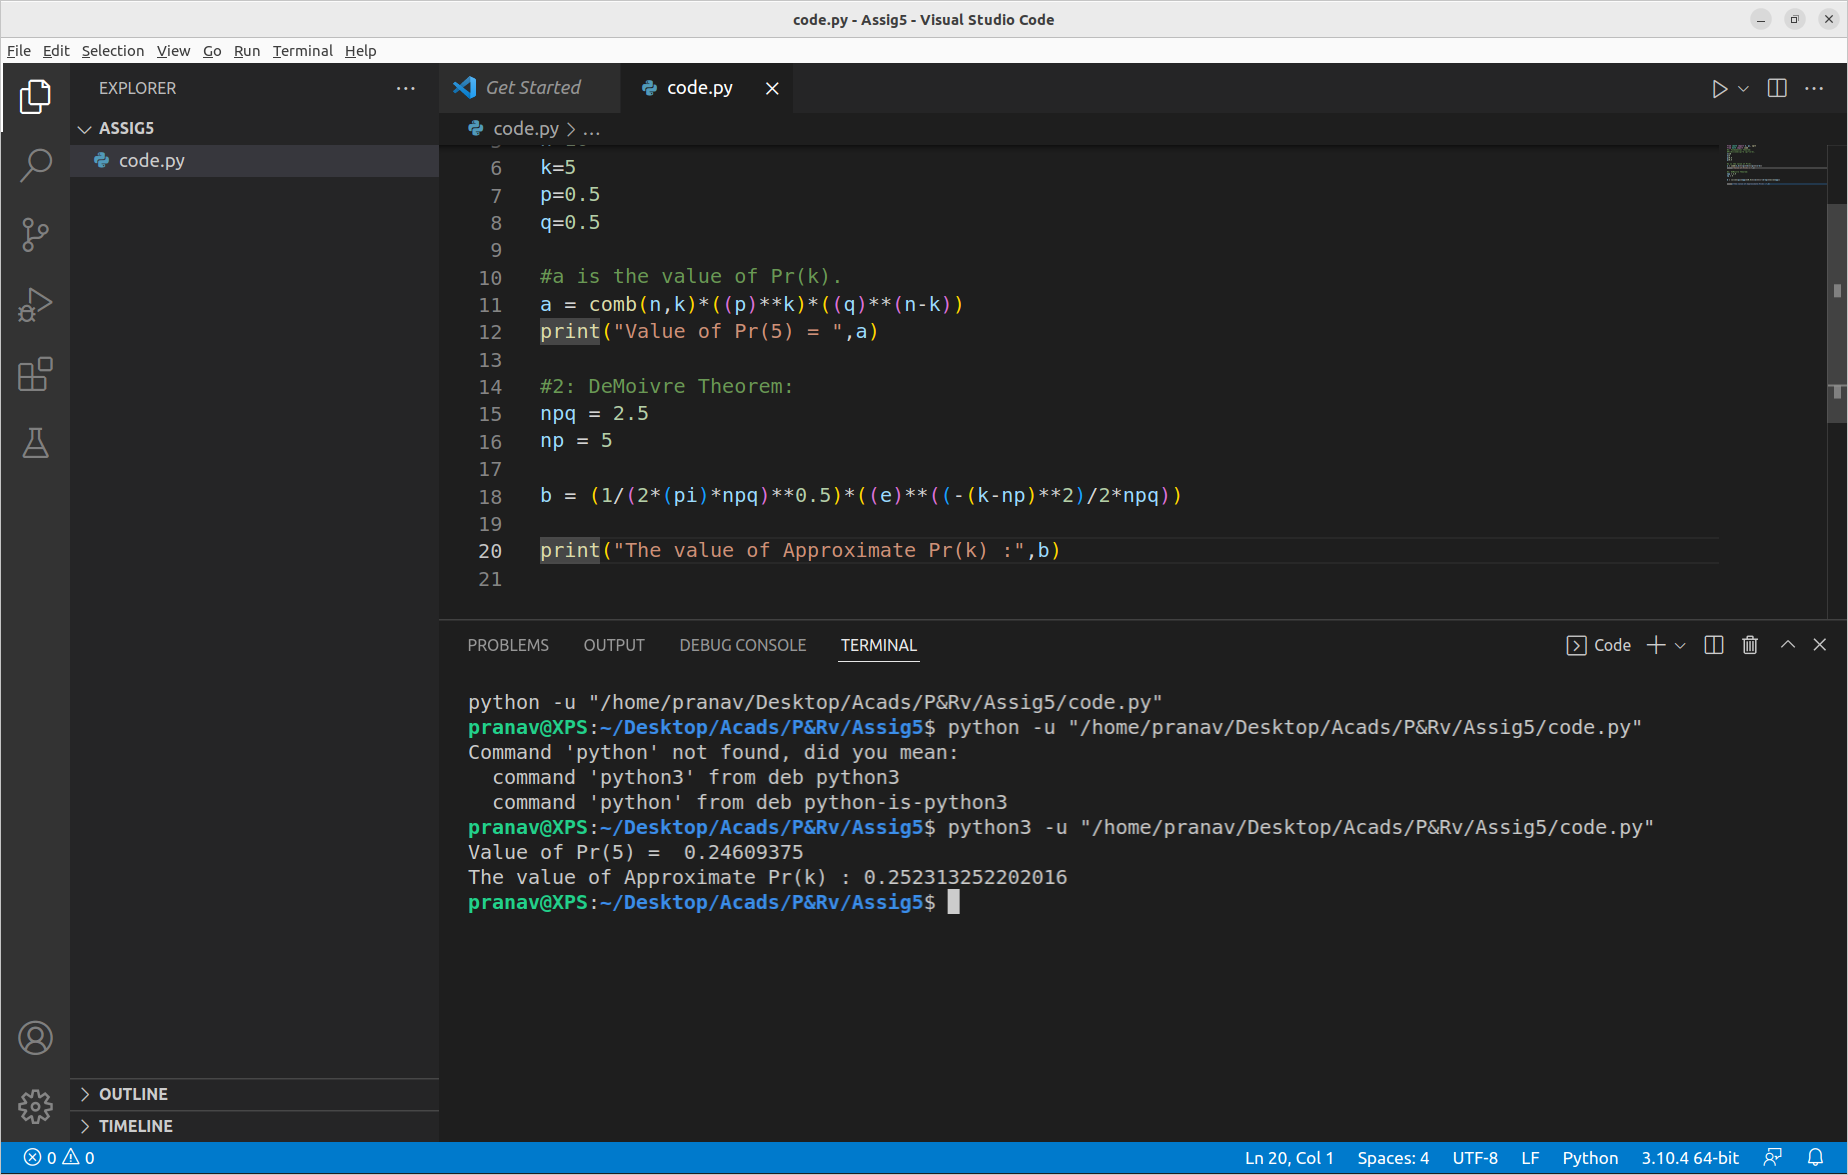
\includegraphics[width=\columnwidth]{figs/output.png}
	%		\caption{Verification Code}
	%		\label{Fig1}	
	%\end{figure}
    \end{frame}
    
    
\end{document}